\documentclass[border=5mm]{standalone}
\usepackage{tikz}
\usepackage{tikz-qtree}

\begin{document}
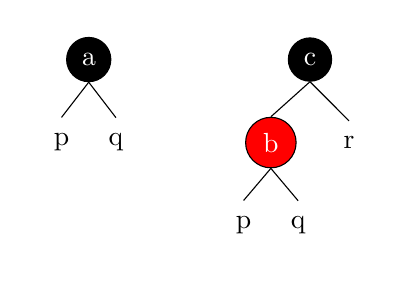
\begin{tikzpicture}[every tree node/.style={align=center}]
    \matrix[row sep=1cm, column sep=1cm] {
    \Tree
    [.\node[draw, fill=black, circle]{\textcolor{white}{a}};
    [.\node[draw=none, circle]{p};]
    [.\node[draw=none, circle]{q};]
    ];
    &
    \Tree
    [.\node[draw, fill=black, circle]{\textcolor{white}{c}};
    [.\node[draw, fill=red, circle]{\textcolor{white}{b}};
    [.\node[draw=none, circle]{p};]
    [.\node[draw=none, circle]{q};]
    ]
    [.\node[draw=none, circle]{r};]
    ]; \\
    };
\end{tikzpicture}
\end{document}
